\chapter{\sffamily Online learning software}

{\bfseries\sffamily Concept.} To outline the software design characteristics of a probabilistic online learning framework, built to interface directly with our generalised simulation engine. The probabilistic algorithms we introduced in the previous chapter will form the basic set of tools in this framework. As well as its own implementations of some learning algorithms, the software is also designed to enable interoperability with other machine learning APIs, e.g., Libtorch (via Gotch), and optimisation libraries, e.g., Gonum and eaopt. For the mathematically-inclined, this chapter will motivate online learning as an essential framework for our use case and how our probabilistic algorithms can work within this context. For the programmers, the software designed and described in this chapter lives in this public Git repository: \href{https://github.com/umbralcalc/learnadex}{https://github.com/umbralcalc/learnadex}.

\section{\sffamily Online learning with any algorithm}

We have discussed the importance of probabilistic learning in the context of environments where only partial state observability is possible and, in the previous chapter, we motivated the use of some specific probabilistic learning methods. However, we haven't yet discussed how we might implement a learning algorithm in practice. In particular, before covering the various aspects of software design, it's important to consider how we want to structure learning by optimisation of an objective with respect to a stream of time series data.

One of the issues that can arise when learning streams of data is `concept drift'. In our context, this would be when the optimal value for $z$ does not match the optimal value at some later point in time. In order to mitigate this, our learning algorithms should be able to track an up-to-date optimal value for $z$ as data is continually passed into them. Iteratively updating the optimal parameters as new data is ingested into the objective function is typically called `online learning'~\cite{hazan2016introduction,sutton2018reinforcement}, in contrast to `offline learning' which would correspond to learning an optimal $z$ only once with the entire dataset provided upfront.

The reader may recall that this book is about building more realistic environments for machine learning systems. An important part of learning from environments in a robust manner is ensuring \emph{adaptability to new data}. In addition to this, stochastic processes are inherently sequential. Many types of system evolve not just their states, but also dynamical description, over time. Online learning is the natural framework to use in this context.

\textcolor{red}{Introduce $y$ as datapoints of $Y$ below here...}

Let's return to the models we discussed in the previous chapter which optimise the cumulative log-likelihood of the data matrix $Y$ with respect to $z$ at a particular point in time, i.e., which optimise $\ln {\cal L}_{{\sf t}+1}(Y\vert z)$ with respect to $z$ at time ${\sf t}+1$. The simplest (and most generally applicable) way to implement an online learning approach with any machnine learning model is to rerun the whole optimisation algorithm for $z$ after each new datapoint has been received using the entire batch of training data with the new addition to it. This kind of `batch' learning will work for most of the standard machine learning algorithms, but the re-training process can take a long time to run in each instance. 

One way to speed things up is to assume that the optimal value for $z$ which was obtained from the previous data iterations is close to the one we will find in the most recent iteration. Hence, by inserting this previous value into the next run of the optimisation procedure as an initial guess, the algorithm will typically converge much more quickly to the optimum. This is more of a practical insight, but are there any quantitative methods which can reduce the amount of computation required to update $z$ when the latest datapoint in the series has been received?

\textcolor{red}{Need to convert the log-likelihood gradient expressions below to be in terms of $y$ instead of $Y$...}

This is where `pure' online learning comes in. When gradients of the log-likelihood are available, we can make things much more efficient. If we denote the $z$ which we have learned from the data up to timestep ${\sf t}$ as $z_*({\sf t})$, we write the following expression for learning from each new datpoint arrival
%%
\begin{align}
z_*({\sf t}+1) &= z_*({\sf t}) - \alpha ({\sf t}+1,\dots ) \frac{\partial}{\partial z} \ln {\cal L}_{{\sf t}+1}(y\vert z) \,,
\end{align}
%%
which is based on a stochastic gradient descent (SGD) algorithm approach. In contrast to the more standard SGD approach --- which would be applied to mini-batches of the data --- this update is applied to $z_*$ using the log-likelihood at each point in time in sequence.

\textcolor{red}{Got to here in rewrite...}
\textcolor{red}{Still need to discuss:
\begin{itemize}
\item{the importance of gradients}
\item{batch learning algorithms --- more like Gaussian processes}
\item{`pure' online learning algorithms --- more like empirical probabilistic reweighting}
\item{introduce the $\beta$ past discounting factor in this section and explain what it's for}
\item{refactor the code so that it's always doing online learning under the hood --- this can either be rolling refits in blocks on a refitting schedule with any optimisation algorithm of choice or full online learning Adam optimisation $$z_*({\sf t}+1) = -\alpha [{\sf t}+1,\text{stats of gradient history like Adam}] \frac{\partial}{\partial z} \ln {\cal L}_{{\sf t}+1} + z_*({\sf t})$$}
\end{itemize}}

Note that other excellent online machine learning frameworks are available --- see, e.g., River~\cite{river} and Vowpal Wabbit~\cite{vowpalwabbit}. The motivation for designing our own probabilistic online learning software is to ensure maximal integration with the stochadex simulation engine. We'll aim to achieve this by designing the code to use the same data structures and and concepts as we used when building the stochadex, where possible. In the next section on software design, we will show how this can be done while still maintaining extensibility and interoperability with other machine learning libraries and APIs. So let's get on with it!

\section{\sffamily Software design}

Let's now take a step back from the specifics of the probabilistic reweighting algorithm to introduce our new sofware package for this part of the book: the `learnadex'. At its core, the learnadex algorithm adapts the stochadex iteration engine to iterate through streams of data in order to accumulate a global objective function value with respect to that data. The user may then choose which optimisation algorithm (or write their own) to use in order to leverage this objective for learning a better representation of the data. 

As we discussed at the end of the last section, the algorithms in the learnadex are all applied in an `online' fashion --- refitting for the optimal hyperparameters $z$ as new data is streamed into them. A challenging aspect of online learning is in managing the computational expense of recomputing the optimal value for $z$ after each new datapoint is sent. To help with this; the user may configure the algorithm recompute the optimum value after larger batches of data have been ingested. The last value of optimum $z$ will also frequently be close to the next optimum in the sequence, so using the former as the initial input into the optimisation routine for the latter is typically very valuable for aiding efficiency.

Reusing the \texttt{PartitionCoordinator} code of the stochadex to facilitate online learning makes neat use of software which has already been designed and tested in earlier chapters of this book. However, in order to fully achieve this, a few minor extensions to the typing structures and code abstractions are necessary; as we show in Fig.~\ref{fig:learnadex-data-types-design}. To start with, we separate out `learning' from the kind of optimiser in the overall config so as to enable multiple optimisation algorithms to be used for the same learning problem. The hyperparameters that define that optimisation problem domain can be determined by the user with an extension to the \texttt{OtherParams} object so that it includes some optional Boolean masks over the parameters, i.e., \texttt{OtherParams.FloatParamMask} and \texttt{OtherParams.IntParamMask}. These masks are used to extract the parameters of interest, which can then be flattened and formatted to fit into any generic optimisation algorithm.

\begin{figure}[h]
\centering
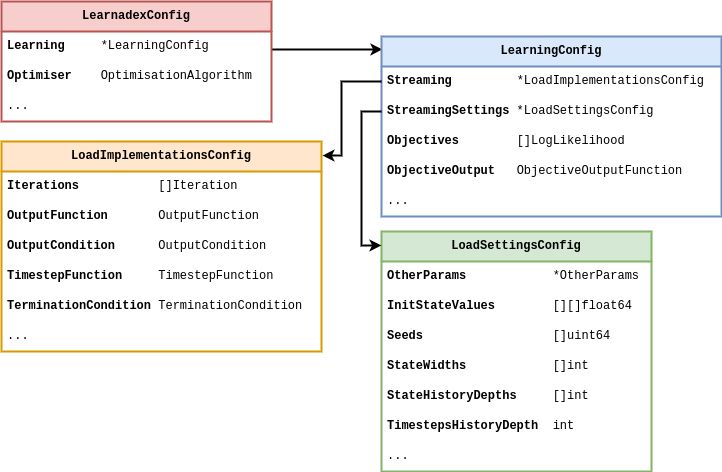
\includegraphics[width=12cm]{images/chapter-3-learnadex-data-types.drawio.png}
\caption{A relational summary of the core data types in the learnadex.}
\label{fig:learnadex-data-types-design}
\end{figure}

On the learning side; in order to define a specific objective for each data iterator to compute while the data streams through it, we have abstracted a `log-likelihood' type. Similarly, each iterator also gets a data streamer configuration which defines where the data is streaming from --- e.g., from a file on disk, from a local database instance or maybe via a network socket --- and also some inherited abstractions from the stochadex which define the time stepping function and when the data stream ends. In Fig.~\ref{fig:learnadex-data-iterator} below, we provide a schematic of the method calls of (and within) each data iterator.

\textcolor{red}{\begin{itemize}
\item{refactor the code and integrate the reweighting algorithm with Libtorch models for the conditional probabilities --- describe how this is supported}
\item{describe the method calls diagram in more detail --- in particular, point out how it can replace the \texttt{Iteration.Iterate} method which is called when the \texttt{StateIterator} is asked for another iteration from the \texttt{PartitionCoordinator} of the stochadex}
\item{then talk about the optimiser! starting with non-gradient-based: the two packages that are supported out of the box are gonum and eaopt (still need to do gago --- see here: github.com/maxhalford/eaopt) }
\item{also need to then support gradient-based algorithms (like vanilla SGD) by implementing Eq.~(\ref{eq:log-likelihood-reweighting-grad}) for the current basic implementations in the learnadex --- shouldn't be too difficult!}
\item{then talk about the output - talk about the possibilities for output and what the default setting to json logs is for}
\item{could also be written to, e.g., a locally-hosted database server and the best-suited would be a NoSQL document database, e.g., MongoDB~\cite{mongodb}, but building something bespoke and simpler is more aligned with the use-case here and with the principles of this book}
\item{describe the need for log exploration and visualisation and then introduce logsplorer - a REST API for querying the json logs (with basic filtering and selection capabilities but could be extended to more advanced options) and optionally also launches a visualisation React app written in Typescript}
\item{note how this could be scaled to cloud services easily and remotely queried through the logsplorer API and visualised} 
\end{itemize}}

\begin{figure}[h]
\centering
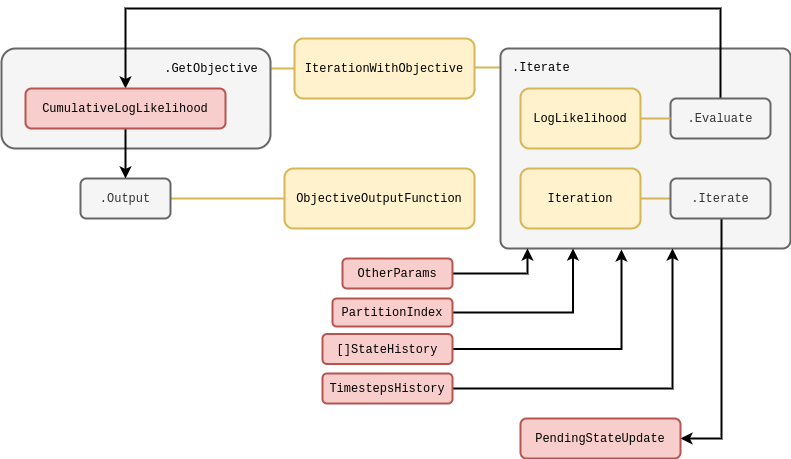
\includegraphics[width=14cm]{images/chapter-3-learnadex-data-iterator.drawio.png}
\caption{A schematic of an iteration with an objective function evaluation.}
\label{fig:learnadex-data-iterator}
\end{figure}

As with the software we wrote for the stochadex, the learnadex main binary executable leverages templating to enable full configurability of all the implementations and settings of Fig.~\ref{fig:learnadex-data-types-design} through passing configs at runtime. Users can alternatively use the learnadex as a library for import, if they desire more control over the code execution. 

\begin{figure}[h]
\centering
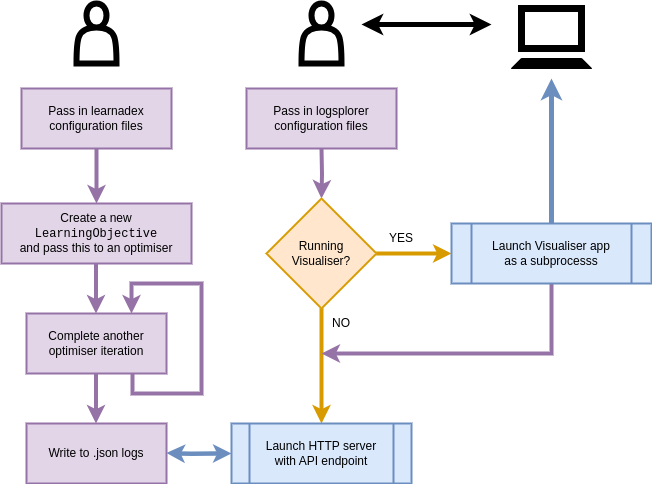
\includegraphics[width=13cm]{images/chapter-3-learnadex-main.drawio.png}
\caption{A diagram of the main learnadex and logsplorer executables.}
\label{fig:learnadex-main}
\end{figure}
    